\section{Aufbau}
\label{sec:Aufbau}
Es wird in diesem Versuch der Zeeman-Effekt an einer Cadmiumlampe im Magnetfeld
eines Elektromagneten untersucht.
Dazu wird die Cd-Lampe zwischen die Polschuhe des Elektromagneten gebracht. Die
Stromstärke kann auf einem externen Ampèremeter abgelesen werden. Um die
magnetische Flussdichte zu messen wird eine Hallsonde in das Magnetfeld gebracht.
Das Licht der Cadmiumlampe wird transversal zum Magnetfeld beobachtet. Dazu ist eine
Optik, wie sie in Abbildung \ref{fig:apparatur} schematisch dargestellt ist notwendig.
Das Objektiv $O$ sorgt dafür, dass das Licht möglichst parallel auf die Kondensorlinse
trifft. Die Kondensorlinse $L_\text{1}$ hat die Aufgabe einen möglichst großen Teil des Lichts
auf den Spalt $S_\text{1}$ zu fokussieren. Diese beiden Linsen haben also die Funktion, dass
das Licht eine möglichst große Intensität hat. Damit das Licht möglicht parallel
in das Geradsichtprisma eintritt befindet sich vor dem Prisma eine Linse $L_\text{2}$
und der Spalt $S_\text{1}$. Durch das Geradsichtprisma kann das Licht der Cd-Lampe
spektral zerlegt werden. Der Unterschied zu einem Prisma besteht darin, dass sich
die Richtung der optischen Achse nicht ändert. Hinter dem Geradsichtprisma befindet sich
der Polarisationsfilter mit dem die Polarisation des Lichtes untersucht werden kann.
Dahinter ist eine Linse $L_\text{3}$ welche das schon spektral aufgespaltene Licht
auf den Spalt $S_\text{2}$ bündelt. Da der Spalt beweglich ist, kann so die zu
untersuchende Spektrallinie ausgewählt werden. In Abbildung \ref{fig:apparatur}
wird die blaue Linie durchgelassen. Mit der vierten Linse $L_\text{4}$
wird das Licht auf den Eintrittsspalt der Lummer-Gehrcke-Platte fokussiert.
Die wesentlichen Bestandteile der Lummer-Gehrke-Platte sind eine planparallele
Glasplatte und ein darauf aufgesetztes Prisma. Mit dieser Platte kann ein hohes
Auflösungsvermögen erreicht werden. Wie in der Abbildung \ref{fig:lummer} zu sehen
ist, wird das Licht innerhalb der planparallelen Platten reflektiert. Die
Lummer-Gehrke-Platte wird so montiert, dass der einfallende Strahl unter einem Winkel
einfällt, der nahe dem der Totalreflexion ist. So tritt bei jeder Reflexion ein
geringer Anteil der Lichts unter einem sehr spitzem Winkel (bezüglich der Platte)
aus der Platte aus. So entstehen viele interferenzfähige Strahlen. Die Bedingung
für konstruktive Interferenz lautet:
\begin{equation}
  2d \cdot \cos(\alpha) = \text{n} \lambda \\.
\end{equation}
Dabei bezeichnet $d$ die Dicke der Platte, $\lambda$ die eingestrahlte Wellenlänge.
Der Gangunterschied der Interferenzstreifen entspricht der eingestrahlten Wellenlänge
$\lambda$. Wenn sich die Cd-Lampe in einem Magnetfeld befindet, verändert sich die
Wellenlänge um $\delta\lambda$. Folglich verschiebt sich auch der Interferenzstreifen
um $\delta s$. Die maximale Differenz zweier Wellenlängen, deren Interferenzmaxima
sich nicht überlagern, ist:
\begin{equation}
  \label{eq:lambda_D}
  \Delta \lambda_\text{D} = \frac{\lambda^2}{2d\sqrt{n^2-1}}
\end{equation}
dies wird als Dispersionsgebiet bezeichnet. Die Lummer-Gehrcke-Platte hat ein
Auflösungsvermögen $A$ von:
\begin{equation}
  \label{eq:Aufloesung}
  A = \frac{\lambda}{\Delta \lambda} = \frac{L}{\lambda}\left(n^2-1\right),
\end{equation}
wobei $L$ die Länge der Platte bezeichnet und $n$ den Brechungsindex
(vgl. Abbildung \ref{fig:lummer}). Hinter der Lummer-Gehrcke-Platte befindet sich eine
Digitalkamera, mit welcher ein Bild von dem Interferenzmuster aufgenommen werden kann.

\begin{figure}
  \centering
  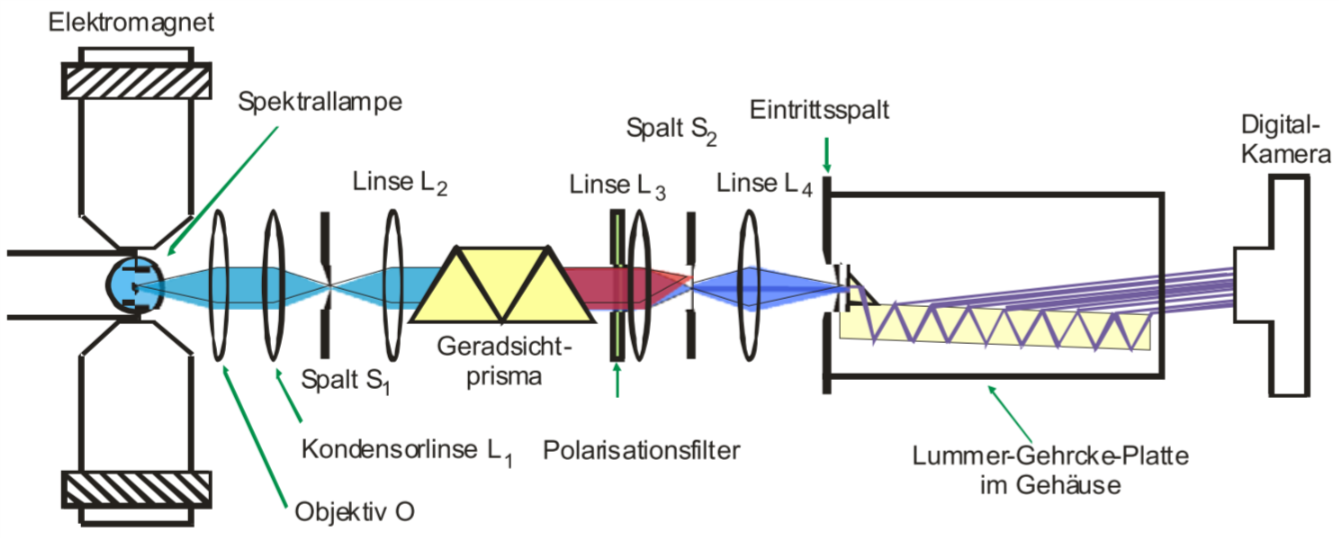
\includegraphics[width=\textwidth]{SchematischApparatur.png}
  \caption{Schematische Darstellung der Apparatur zur Beobachtung des Zeeman-Effekts \cite{sample}.}
  \label{fig:apparatur}
\end{figure}

\begin{figure}
  \centering
  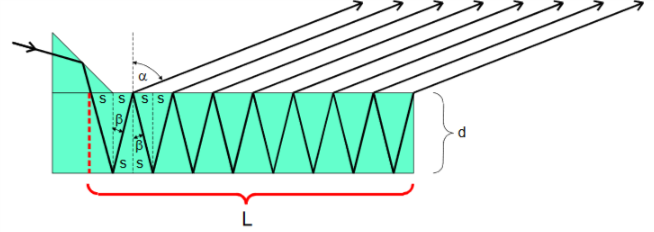
\includegraphics[width=0.7\textwidth]{Lummer.png}
  \caption{Schematische Darstellung des Strahlengangs innerhalb der Lummer-Gehrcke-Platte \cite{sample}.}
  \label{fig:lummer}
\end{figure}




\section{Durchführung}
\label{sec:Durchführung}
Bevor mit dem eigentlichem Versuch begonnen wird, muss der Elektromagnet geeicht werden.
Dies geschieht, indem die Hallsonde in das Magnetfeld gebracht wird und das $B$-Feld
in Abhängigkeit von der Stromstärke notiert wird.\\
\\
Der Versuch wird wie in Abschnitt \ref{sec:Aufbau} beschrieben aufgebaut. Es wird
lediglich der Polarisationsfilter noch nicht eingebaut. Die
verschiedenen optischen Komponenten können in ihrer Position variiert werden.
Zunächst sollten das Objektiv $O$ und die Linse $L_\text{1}$ solange verschoben
werden, bis sie ein möglicht scharfes und intensives Lichtbündel auf den
Spalt $S_\text{1}$ bringen. Die zweite Linse $L_\text{2}$ wird so angebracht, dass
ein paralleles Lichtbündel auf das Geradsichtprisma trifft. Das Lichtbündel
sollten ungefähr die gleiche Größe wie das Prisma haben. Die dritte Linse wird so
angebracht, dass auf dem Spalt $S_\text{2}$ ein scharfes Linienspektrum zu erkennen ist.
Mit dem Spalt kann nun eine Linie aus dem Spektrum ausgewählt werden. Für die
Justierung empfiehlt es sich mit der grünen Linie anzufangen, die aus einem
Quecksilberanteil in der Lampe stammt, da das Auge für diese besonders empfindlich ist.
Mit der vierten Linse $L_\text{4}$ wird das Licht auf das Prisma
der Lummer-Gehrcke-Platte fokussiert. Der Strahl sollte nahezu senkrecht auf die
Fläche des Prismas treffen um Reflexionen zu vermeiden. Die planparallele
Glasplatte sollte in einem möglichst
spitzen Winkel gegenüber der ursprünglichen Strahlrichtung sein. Bei der Kamera
muss manuell fokussiert werden. Die Brennweite wird auf unendlich gestellt, da
parallele Strahlen auf die Kamera treffen. Durch die Kamera
werden die Spektrallinien beobachtet. Die Lummer-Gehrrcke-Platte wird solange
gedreht bis auf dem Bildschirm der Kamera die Spektrallinien sichtbar sind. Dabei muss
die Platte sehr vorsichtig gedreht werden, da diese sehr winkelanfällig ist.
Nun wird der Polarisator in den Strahlengang gemäß Abbildung \ref{fig:apparatur}
eingbracht. Je nach Stellung des Polarisators wird der Übergang bei dem $\Delta m = \pm 1$
ist oder $\Delta m = 0$ ist ausgeblendet. Nun werden zwei Bilder gemacht. Einmal
ohne Magnetfeld und einmal mit Magnetfeld. Durch die Drehung des Polarisationsfilters
kann nun festgestellt werden, welche Linien die $\sigma$-Linien und welche die
$\pi$-Linien sind. Um möglichst gute Bilder zu erhalten werden am besten mehrere Bilder
aufgenommen mit unterschiedlichen Belichtungszeiten.\\
\\
Anschließend wird die blaue Linie näher betrachtet. Dazu muss der Spalt $S_\text{2}$
verschoben werden. Und infolge diese Änderung müssen alle nachfolgenden optischen
Instrumente neu justiert werden. Mit der Kamera wird ein Bild ohne Magnetfeld benötigt.
Zusätzlich werden zwei weitere Bilder bei unterschiedlichen Magnetfeldern benötigt.
Und zwar bei solchen Feldern wo einmal die $\pi$-Aufspaltung sichtbar ist und bei
einem anderen Feld die $\sigma$-Aufspaltung.
